 %!TEX root = main.tex
\section*{Results}
\subsection*{Fundamental elements of formulating rank percentile indicators}
Four fundamental elements to calculate the rank percentile indicators are (1) entity; (2) benchmark; (3) metric; and (4) age. The entity specifies the target of interest. For example, it can be a publication (P) or a scholar (S). The benchmark (b) characterizes the individuals that the entity is compared against. For instance, the benchmark can be all the publications in computer science. It can also be the faculty members in a department competing for tenure decisions. The metric (m) specifies the way that the entity is evaluated. For example, it can be the number of citations or h-index. Finally, the age (t) is the number of years that the entity has been alive. The age of a publication is the number of years since it was published, while the age of a scholar is the number of years since his/her first paper was published. By combining these four elements, we use P$_{jt}^{m}(b)$ and S$_{it}^{m}(b)$ to denote the rank percentile indicators for publication $j$ and scholar $i$, respectively. 

\subsection*{The framework of calculating rank percentile indicators}
Suppose the benchmark b contains $N$ publications across $T$ years. For each publication $j\in\{1,\cdots,N\}$, we have a history of some evaluation metric m$_{jt}$ (m$_{jt} \ge 0$) at each age $t=1,\cdots,T_j$ where $T_j$ denotes the total number of years since it's published. The rank percentile indicator of publication $j$ at age $t^\star$, P$_{jt^\star}^{m}(b)$, is computed as follows:
\begin{enumerate}[label=(\arabic*)]
    \item Consider all the $N_{t^\star}$ publications that have $T_j \ge t^\star$, and calculate the rank r$_{jt^\star}$ of publication $j$ based on its metric m$_{jt^\star}$. An average rank is assigned to $r_{jt^\star}$ if there exist other publications that have the same metric value as m$_{jt^\star}$. 
    \item The rank percentile is given by
        \begin{equation}
        \label{eq:rp_rank}
            \text{P}_{j t^\star}^{m}(b) = 
                \begin{cases} 
                    0, & \mbox{if } \text{m}_{j t^\star}=0, \\ 
                    (\text{r}_{j t^\star}-0.5)/N_{t^\star}, & \mbox{otherwise}.
                \end{cases}
        \end{equation}
\end{enumerate}
With the compromise $0.5/N_{t^\star}$ in \eqref{eq:rp_rank}, the median paper will be assigned $50\%$ percentile, and the tails of the citation distribution are treated symmetrically\supercite{allen1914storage}.

The above framework can be easily adapted to compute the rank percentile indicators for scholar $i$ at age $t^\star$, S$_{jt^\star}^{m}(b)$. Furthermore, it is flexible in terms of the choice of the evaluation metric and benchmark. In this paper, we study two benchmarks. The first contains all the scholars in our dataset that come from various disciplines, different institutes and have different starting points of careers. The second benchmark only includes scholars in the area of biological science. Meanwhile, we consider two common choices of the evaluation metric, that are the number of citations (c) and h-index (h). The following are the indicators considered in this paper.
\begin{itemize}
    \item rank percentile indicator for publication $j$:
    \begin{itemize}
        \item \textbf{P$_{jt}^c(b)$}: $m_{jt}$ is the total citations $c_{jt}$ that the paper receives by age $t$,
    \end{itemize}
    \item rank percentile indicator for scholar $i$:
    \begin{itemize}
        \item \textbf{S$_{it}^c(b)$}: $m_{it}$ is the total citations $c_{it}$ that the scholar receives by age $t$.
        \item \textbf{S$_{it}^h(b)$}: $m_{it}$ is the h-index $h_{it}$ of the scholar at age $t$.
        \item \textbf{S$_{it}^{P5}(b)$}: $m_{it} = \sum_{j=1}^{N_t^{(i)}} \text{P}_{j5}^c(b)$, where $N_t^{(i)}$ denotes the total number of papers that the scholar publishes by age $t$. For paper with ages less than $5$, i.e. $T_j<5$, we take the most recent performance P$_{jT_j}^c(b)$ instead. 
    \end{itemize}
\end{itemize}

The rank percentile indicators are highly interpretable. For instance, P$_{jt}^c(b)=0.9$, immediately tells us that paper $j$ performs better than $90 \%$ of the papers in the benchmark at age $t$. Furthermore, two papers from different benchmarks, such as different fields, are directly comparable using the rank percentile indicators. 

\subsection*{The stableness of the rank percentile indicators}
The benchmarks that we study in this paper do not restrict the publications to have the same publishing year or the scholars to have the same starting year of their careers. In many situations, we would like to examine a scholar's performance relative to cohorts that are more senior to her. For instance, to make a promotion decision about a candidate who is in the sixth year of her academic career, the committee may compare her with all other faculty members of the department in the sixth year of their academic careers. The comparison will not be valid, if the candidate is more likely to attract citations than her senior colleagues who start their careers many years before. It may well be the academic environment that results in a better performance of the candidate, rather than the internal factors such as the creativity and productivity. 

Figure \ref{fig:stableness_rp} shows P$_{j 10}^c$ grouped by the publishing years and S$_{i 10}^{P5}$ grouped by the starting year of academic careers, where the benchmark contains all the tenured scholars in our dataset. We see that both indicators are reasonably stable over the physical years. We do not see the pattern that papers or scholars attract more citations than those years before, supporting the validity of rank percentile indicators.

\begin{figure}[ht!]
    \centering
    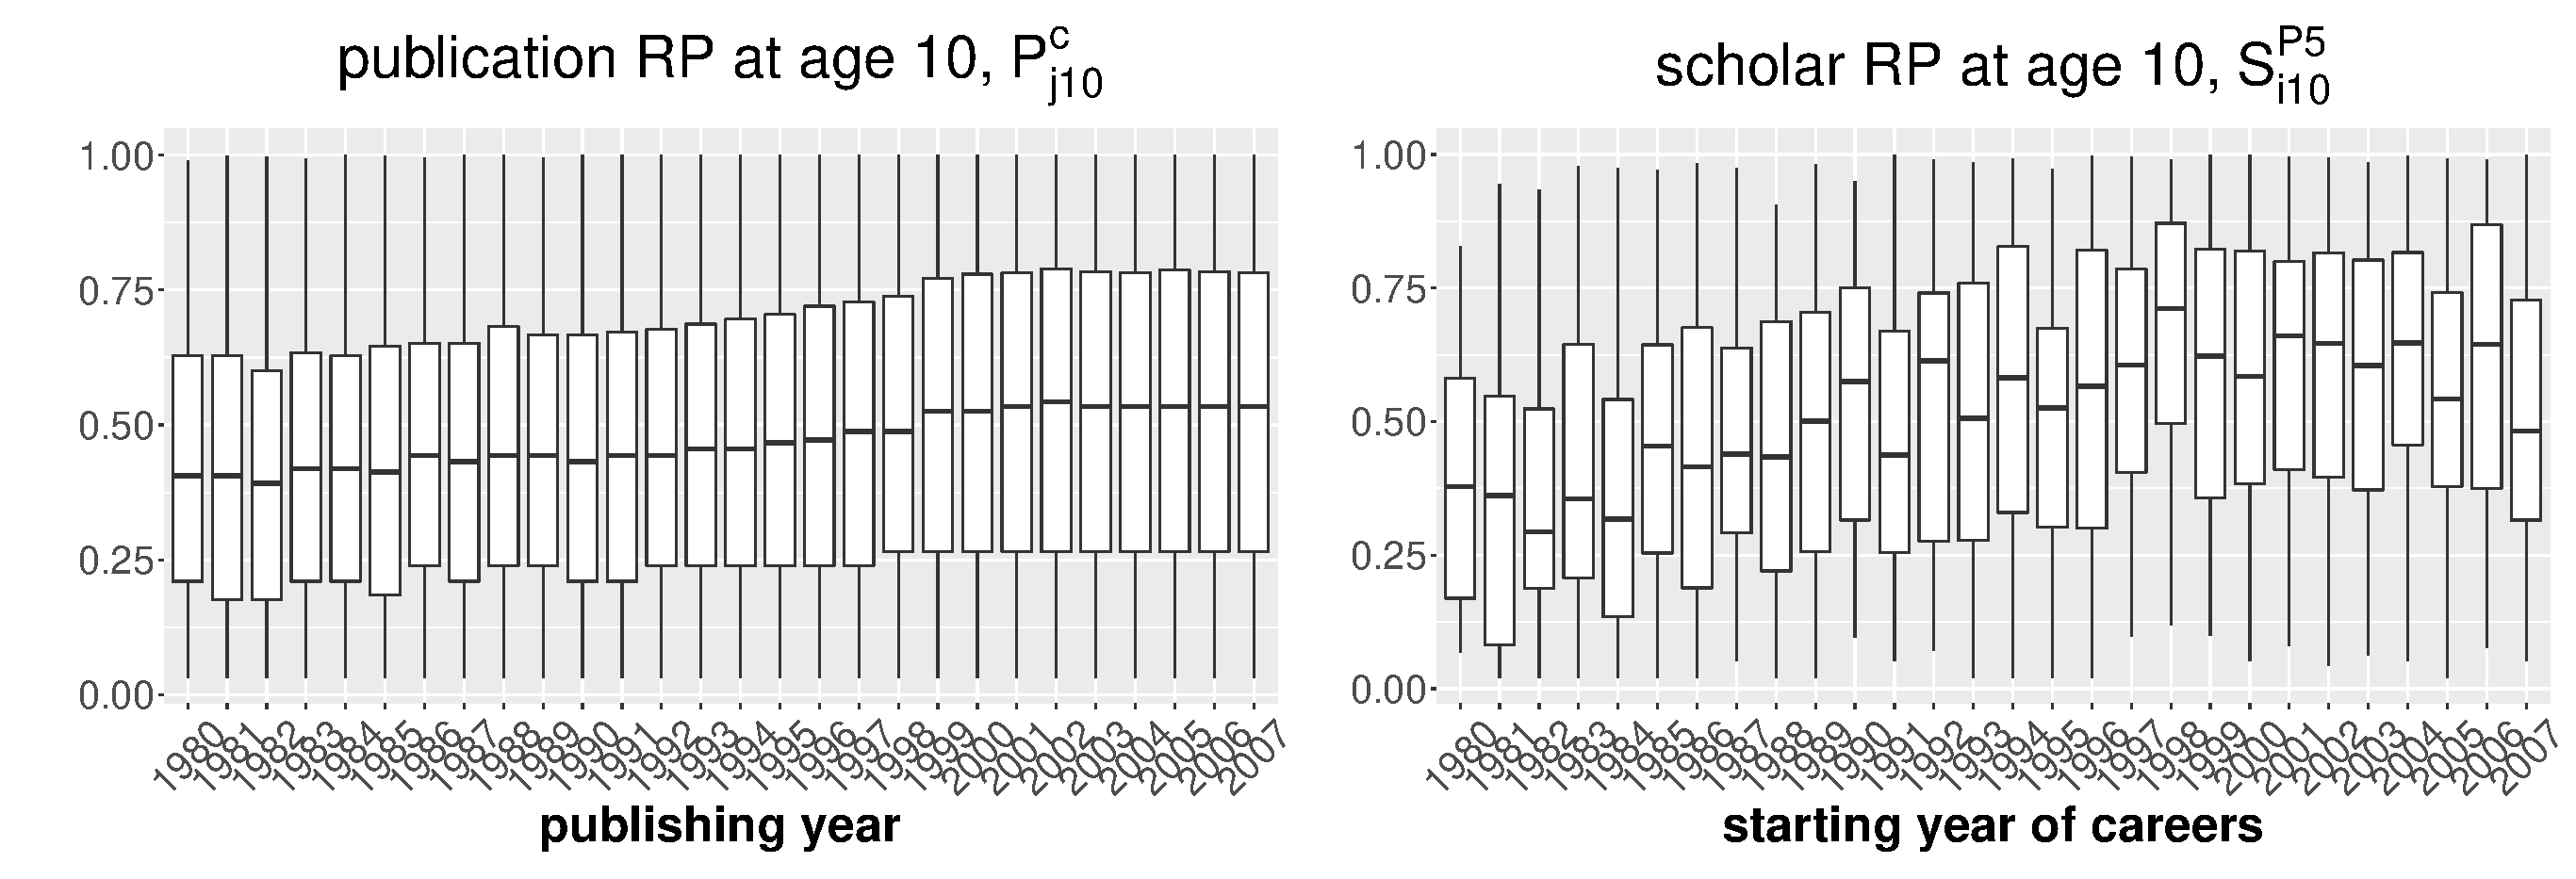
\includegraphics[width=\textwidth]{figures/exploratory/stationarity.eps}
    \caption{P$_{j10}^c$ grouped by the publishing years and and S$_{i10}^{P5}$ grouped by the starting years of academic careers. The benchmark contains professors from various disciplines who receive their tenureships no later than year $2016$.}
    \label{fig:stableness_rp}
\end{figure}

\subsection*{The predictability of the rank percentile indicators}
% publication rank percentile vs citations, predictability, Wang(2013)
\begin{figure}[ht!]
     \centering
     \begin{subfigure}[b]{0.48\textwidth}
         \centering
         \includegraphics[width=\textwidth]{figures/pred_power/ncit_vs_pubrp/cit_age.pdf}
         \caption{}
         \label{fig:pred_cit_age}
     \end{subfigure}
     \hfill
     \begin{subfigure}[b]{0.48\textwidth}
         \centering
         \includegraphics[width=\textwidth]{figures/pred_power/ncit_vs_pubrp/rp_age.pdf}
         \caption{}
         \label{fig:pred_rp_age}
     \end{subfigure}
     \hfill
     \begin{subfigure}[b]{0.48\textwidth}
         \centering
         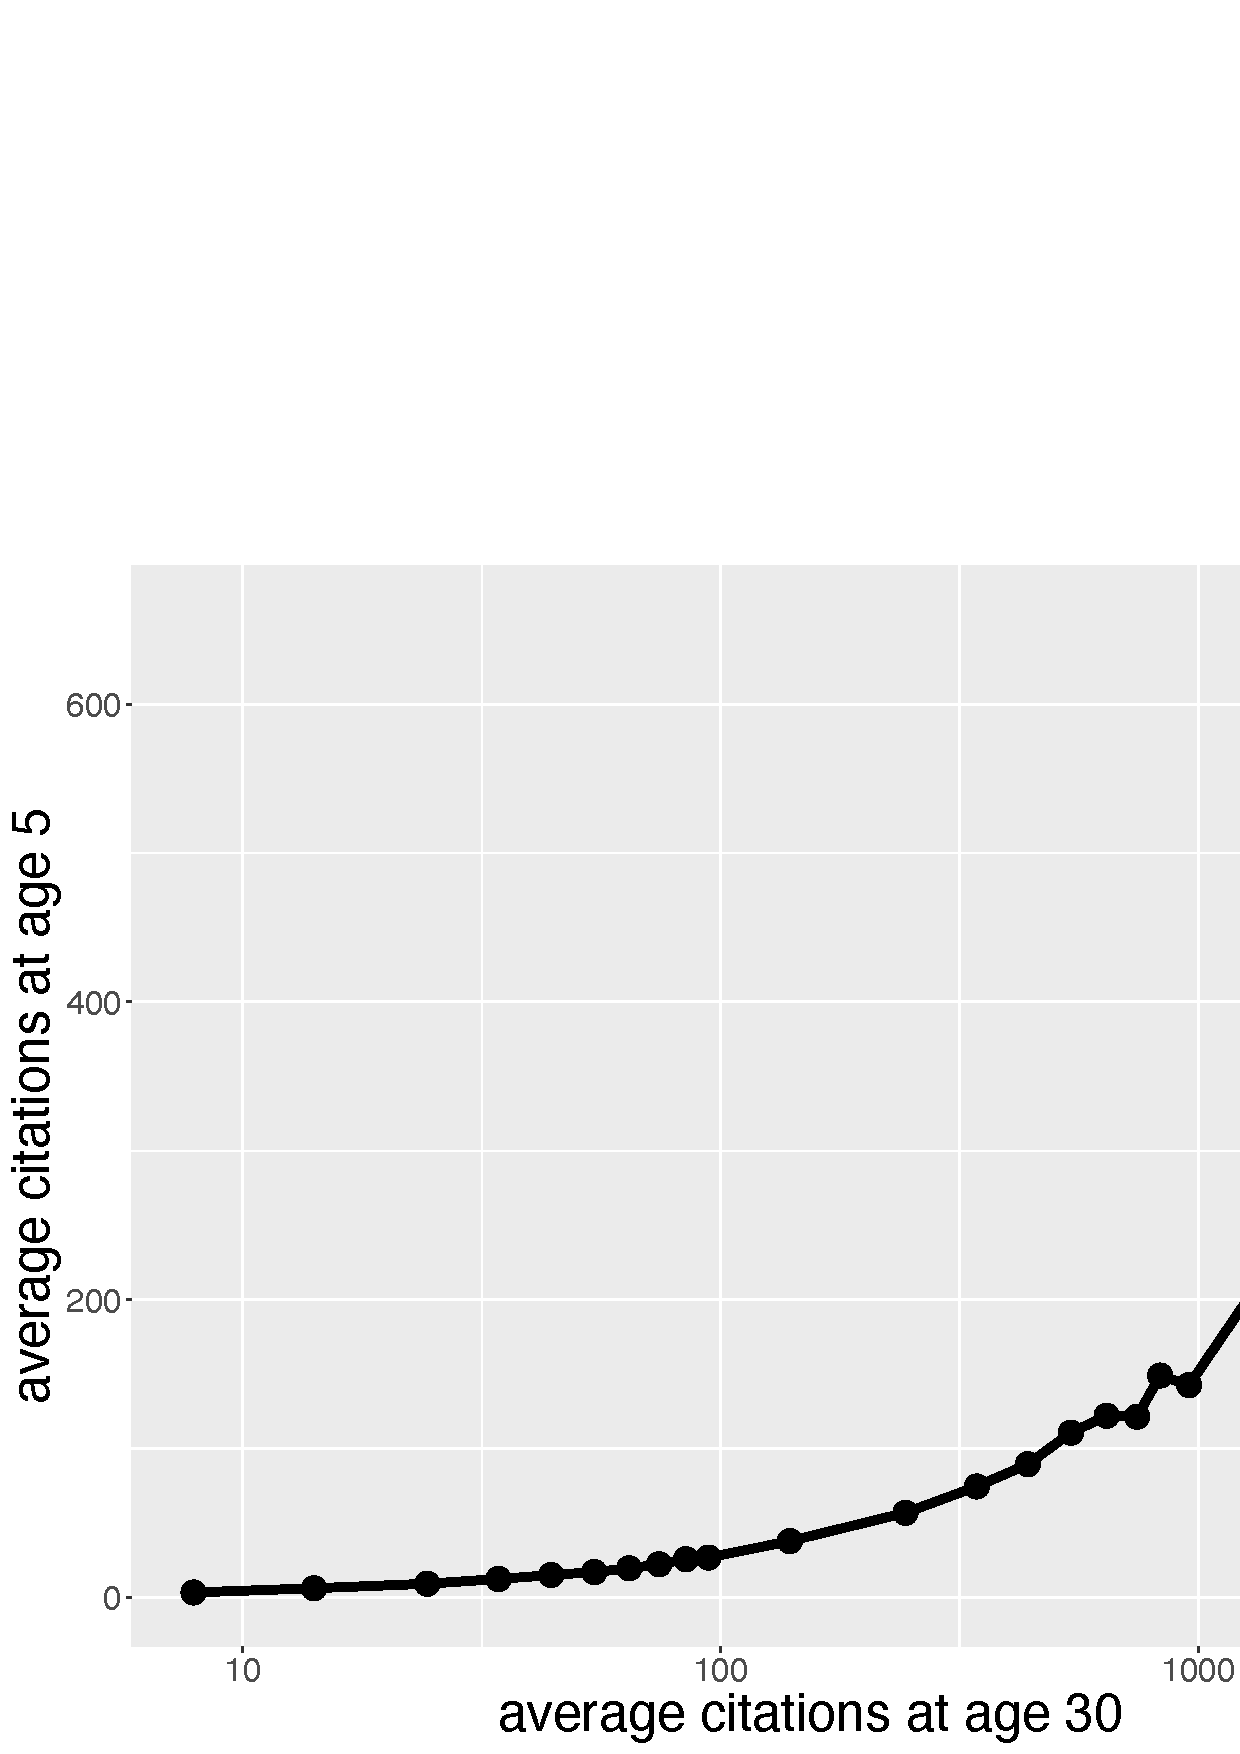
\includegraphics[width=\textwidth]{figures/pred_power/ncit_vs_pubrp/cit_cit.pdf}
         \caption{}
         \label{fig:pred_cit_cit}
     \end{subfigure}
     \hfill
     \begin{subfigure}[b]{0.48\textwidth}
         \centering
         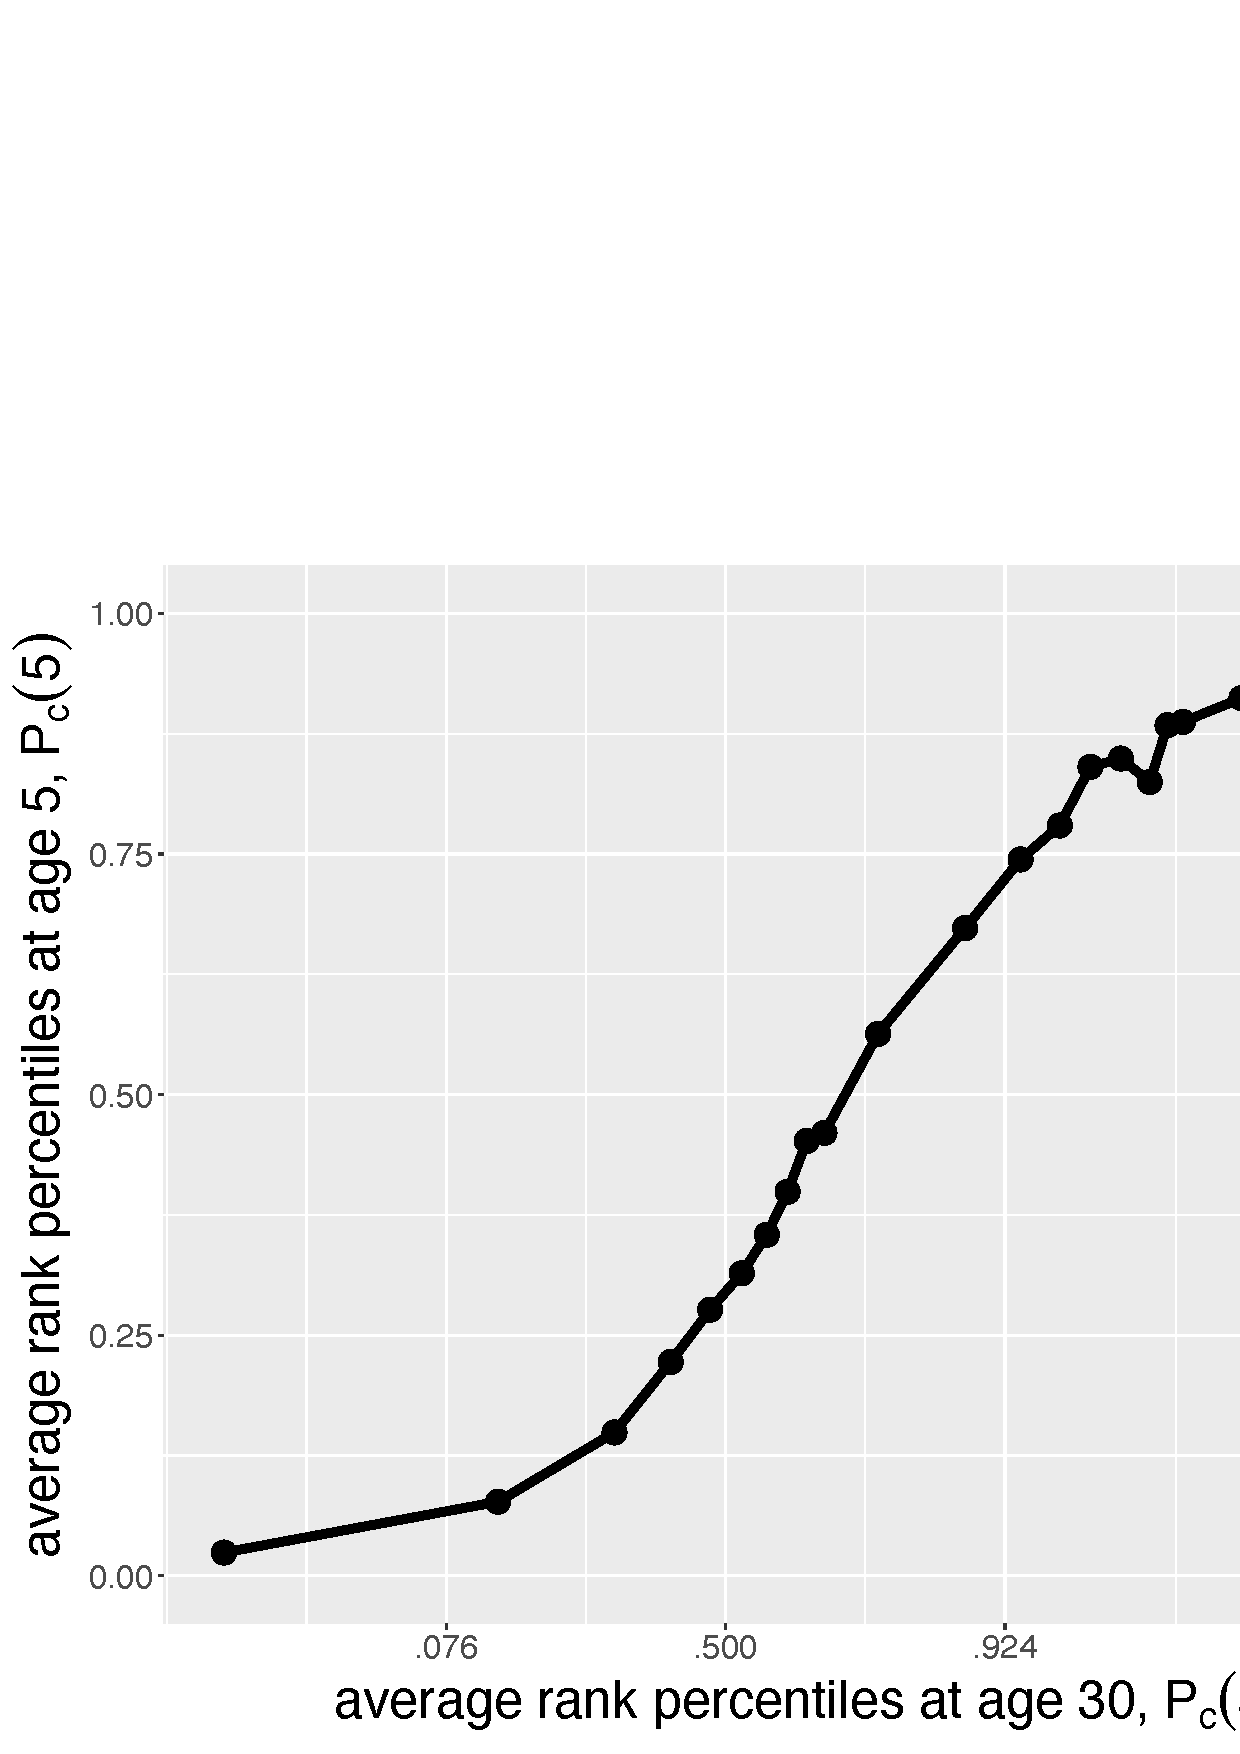
\includegraphics[width=\textwidth]{figures/pred_power/ncit_vs_pubrp/rp_rp.pdf}
         \caption{}
         \label{fig:pred_rp_rp}
     \end{subfigure}
        \caption{The predictability of citations and rank percentiles. The benchmark here is biology. Figure \ref{fig:pred_cit_age} and \ref{fig:pred_rp_age} show the citations and the corresponding rank percentiles for papers that have $50$ citations by age $5$. Figure \ref{fig:pred_cit_cit} displays the average citations by age $5$ over the average citations by age $30$, for different sets of publications, which are pre-specified by dividing the range of $\bar{c}_{j 30}$ into equal intervals in the log scale. Figure \ref{fig:pred_rp_rp} shows the corresponding average rank percentiles for the same sets of publications. Note that we do not claim originality for these plots, as figures \ref{fig:pred_cit_age} and \ref{fig:pred_cit_cit} have been illustrated via a different dataset\supercite{Wang2013}.}
        \label{fig:pub_cit_rp_pred}
\end{figure}


% publication rank percentile, heat map of correlations
\begin{figure}[ht!]
    \centering
    \begin{subfigure}[b]{0.8\textwidth}
        \centering
             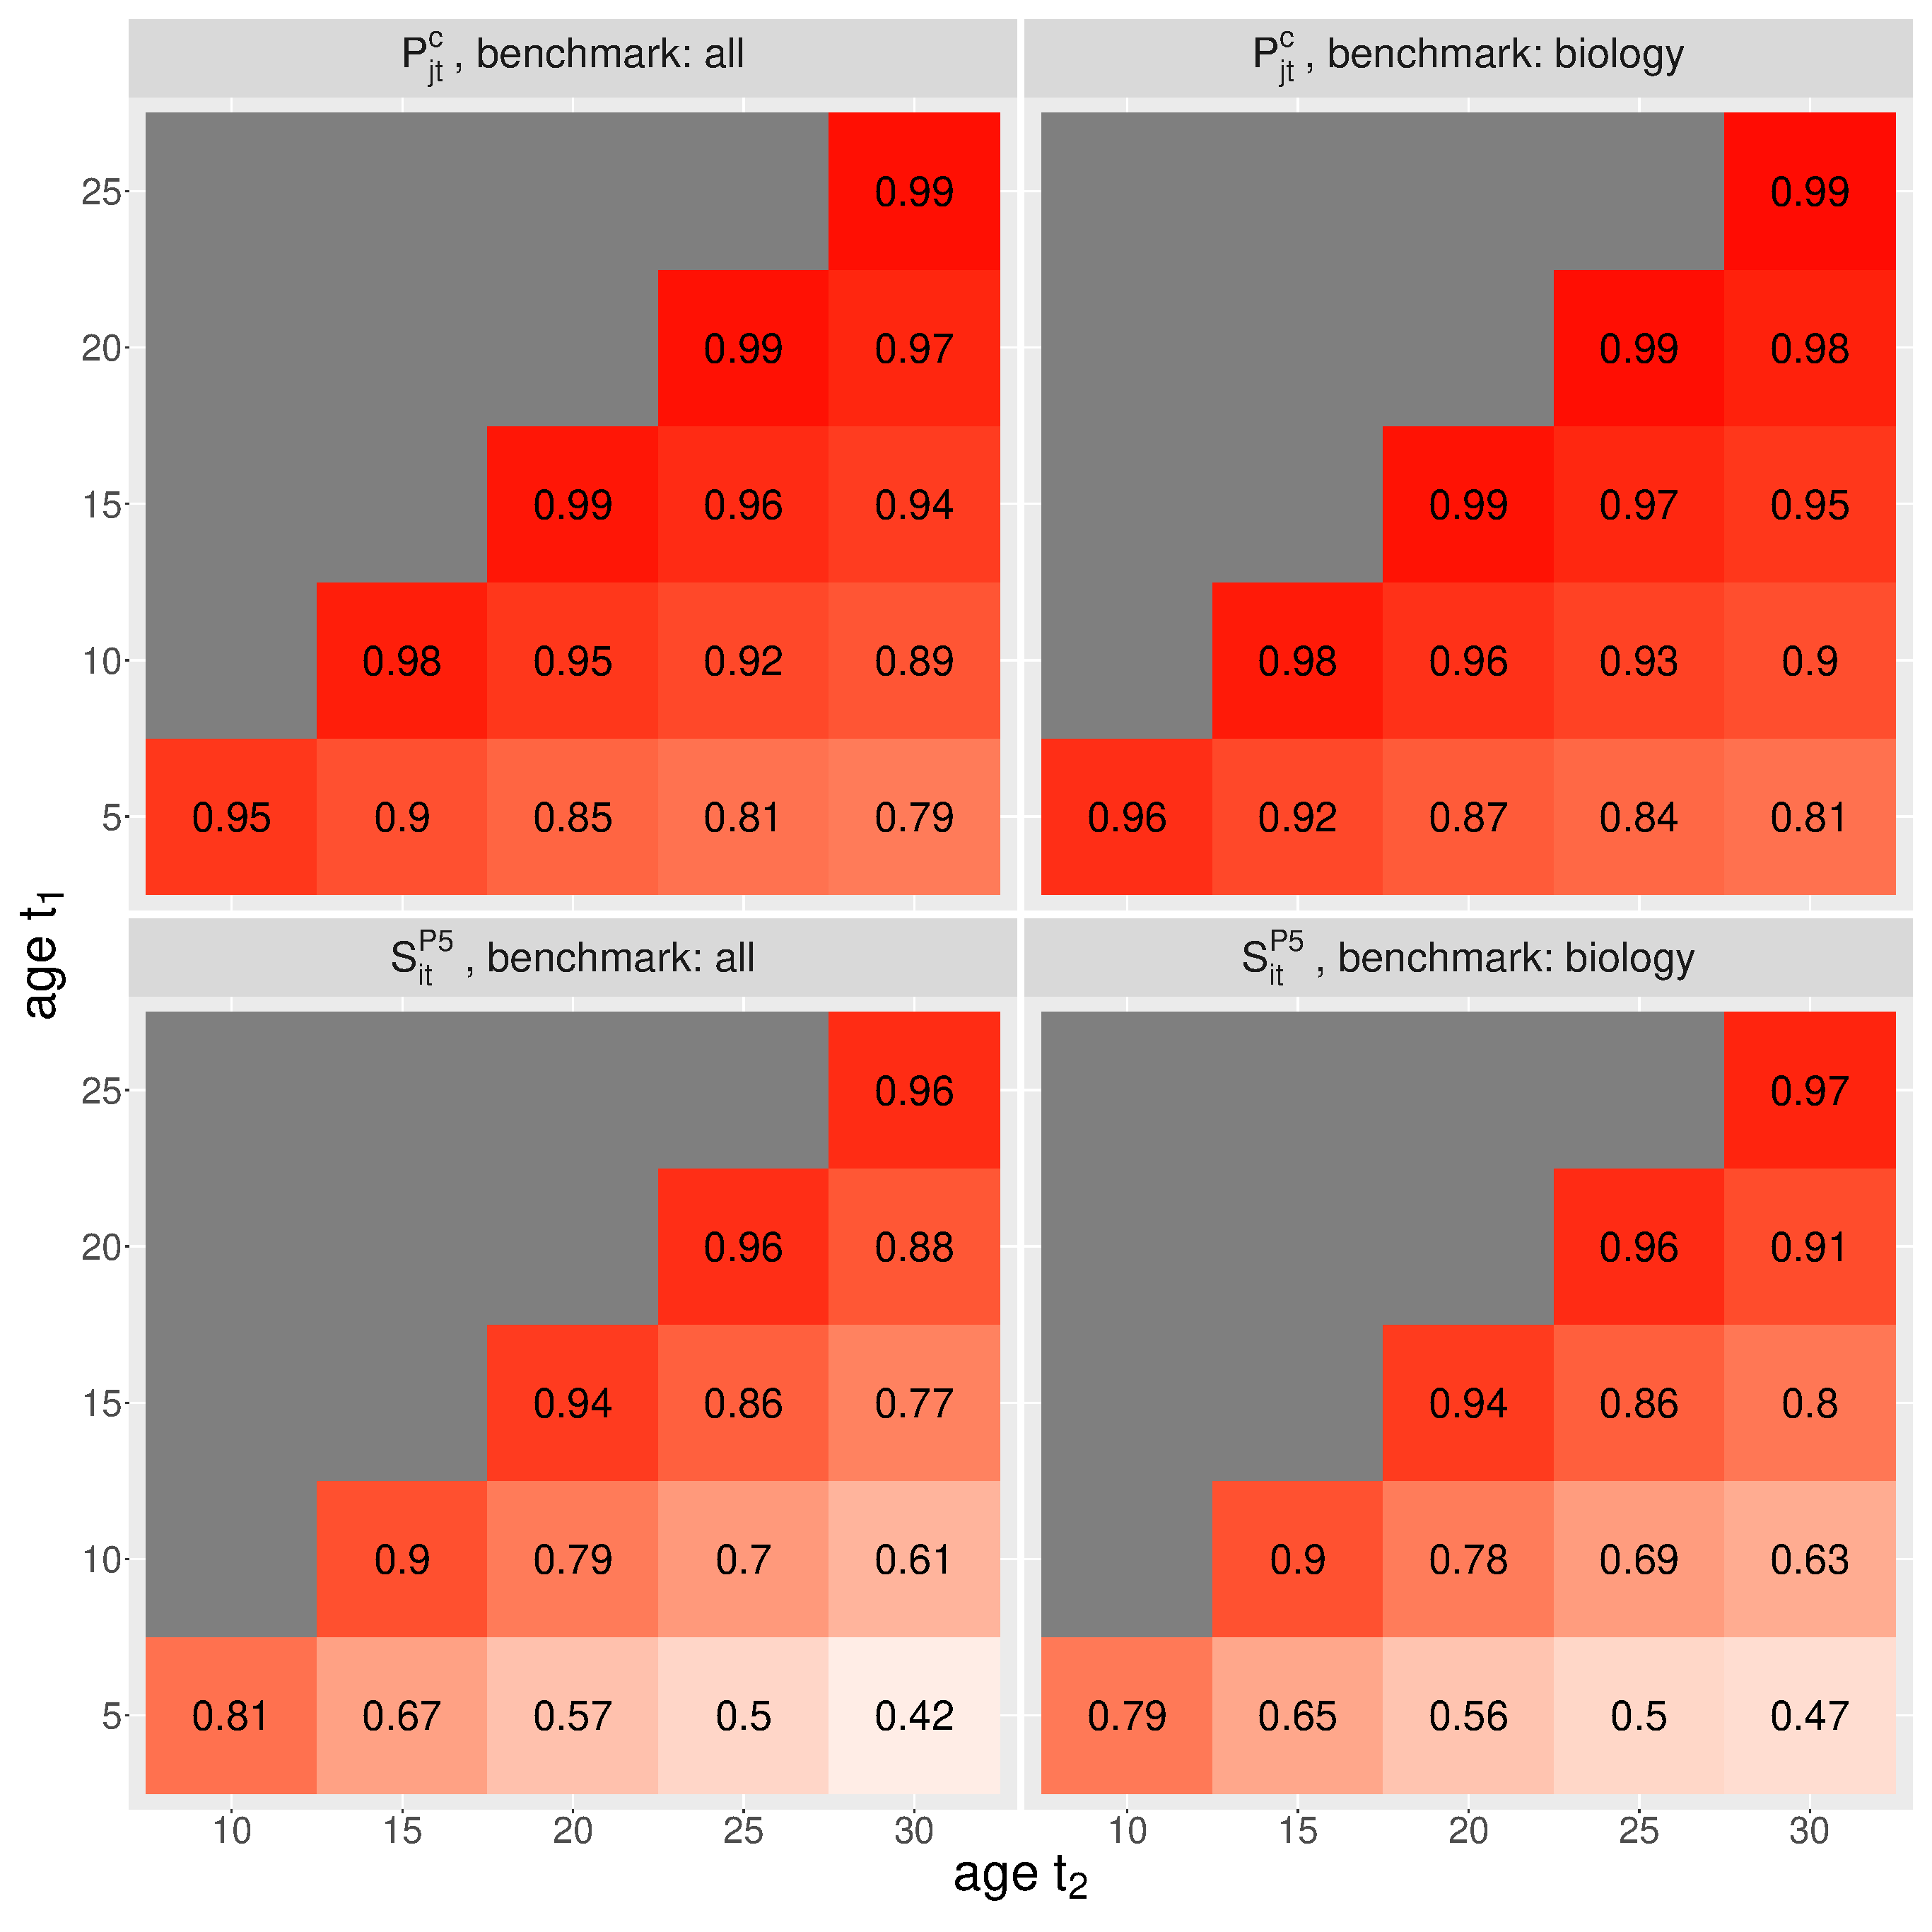
\includegraphics[width=\textwidth]{figures/pred_power/current/heatmap_cor.eps}
         \caption{Predict the cumulative impacts}
         \label{fig:hm_rp_current}
    \end{subfigure}
    
    \begin{subfigure}[b]{0.8\textwidth}
        \centering
             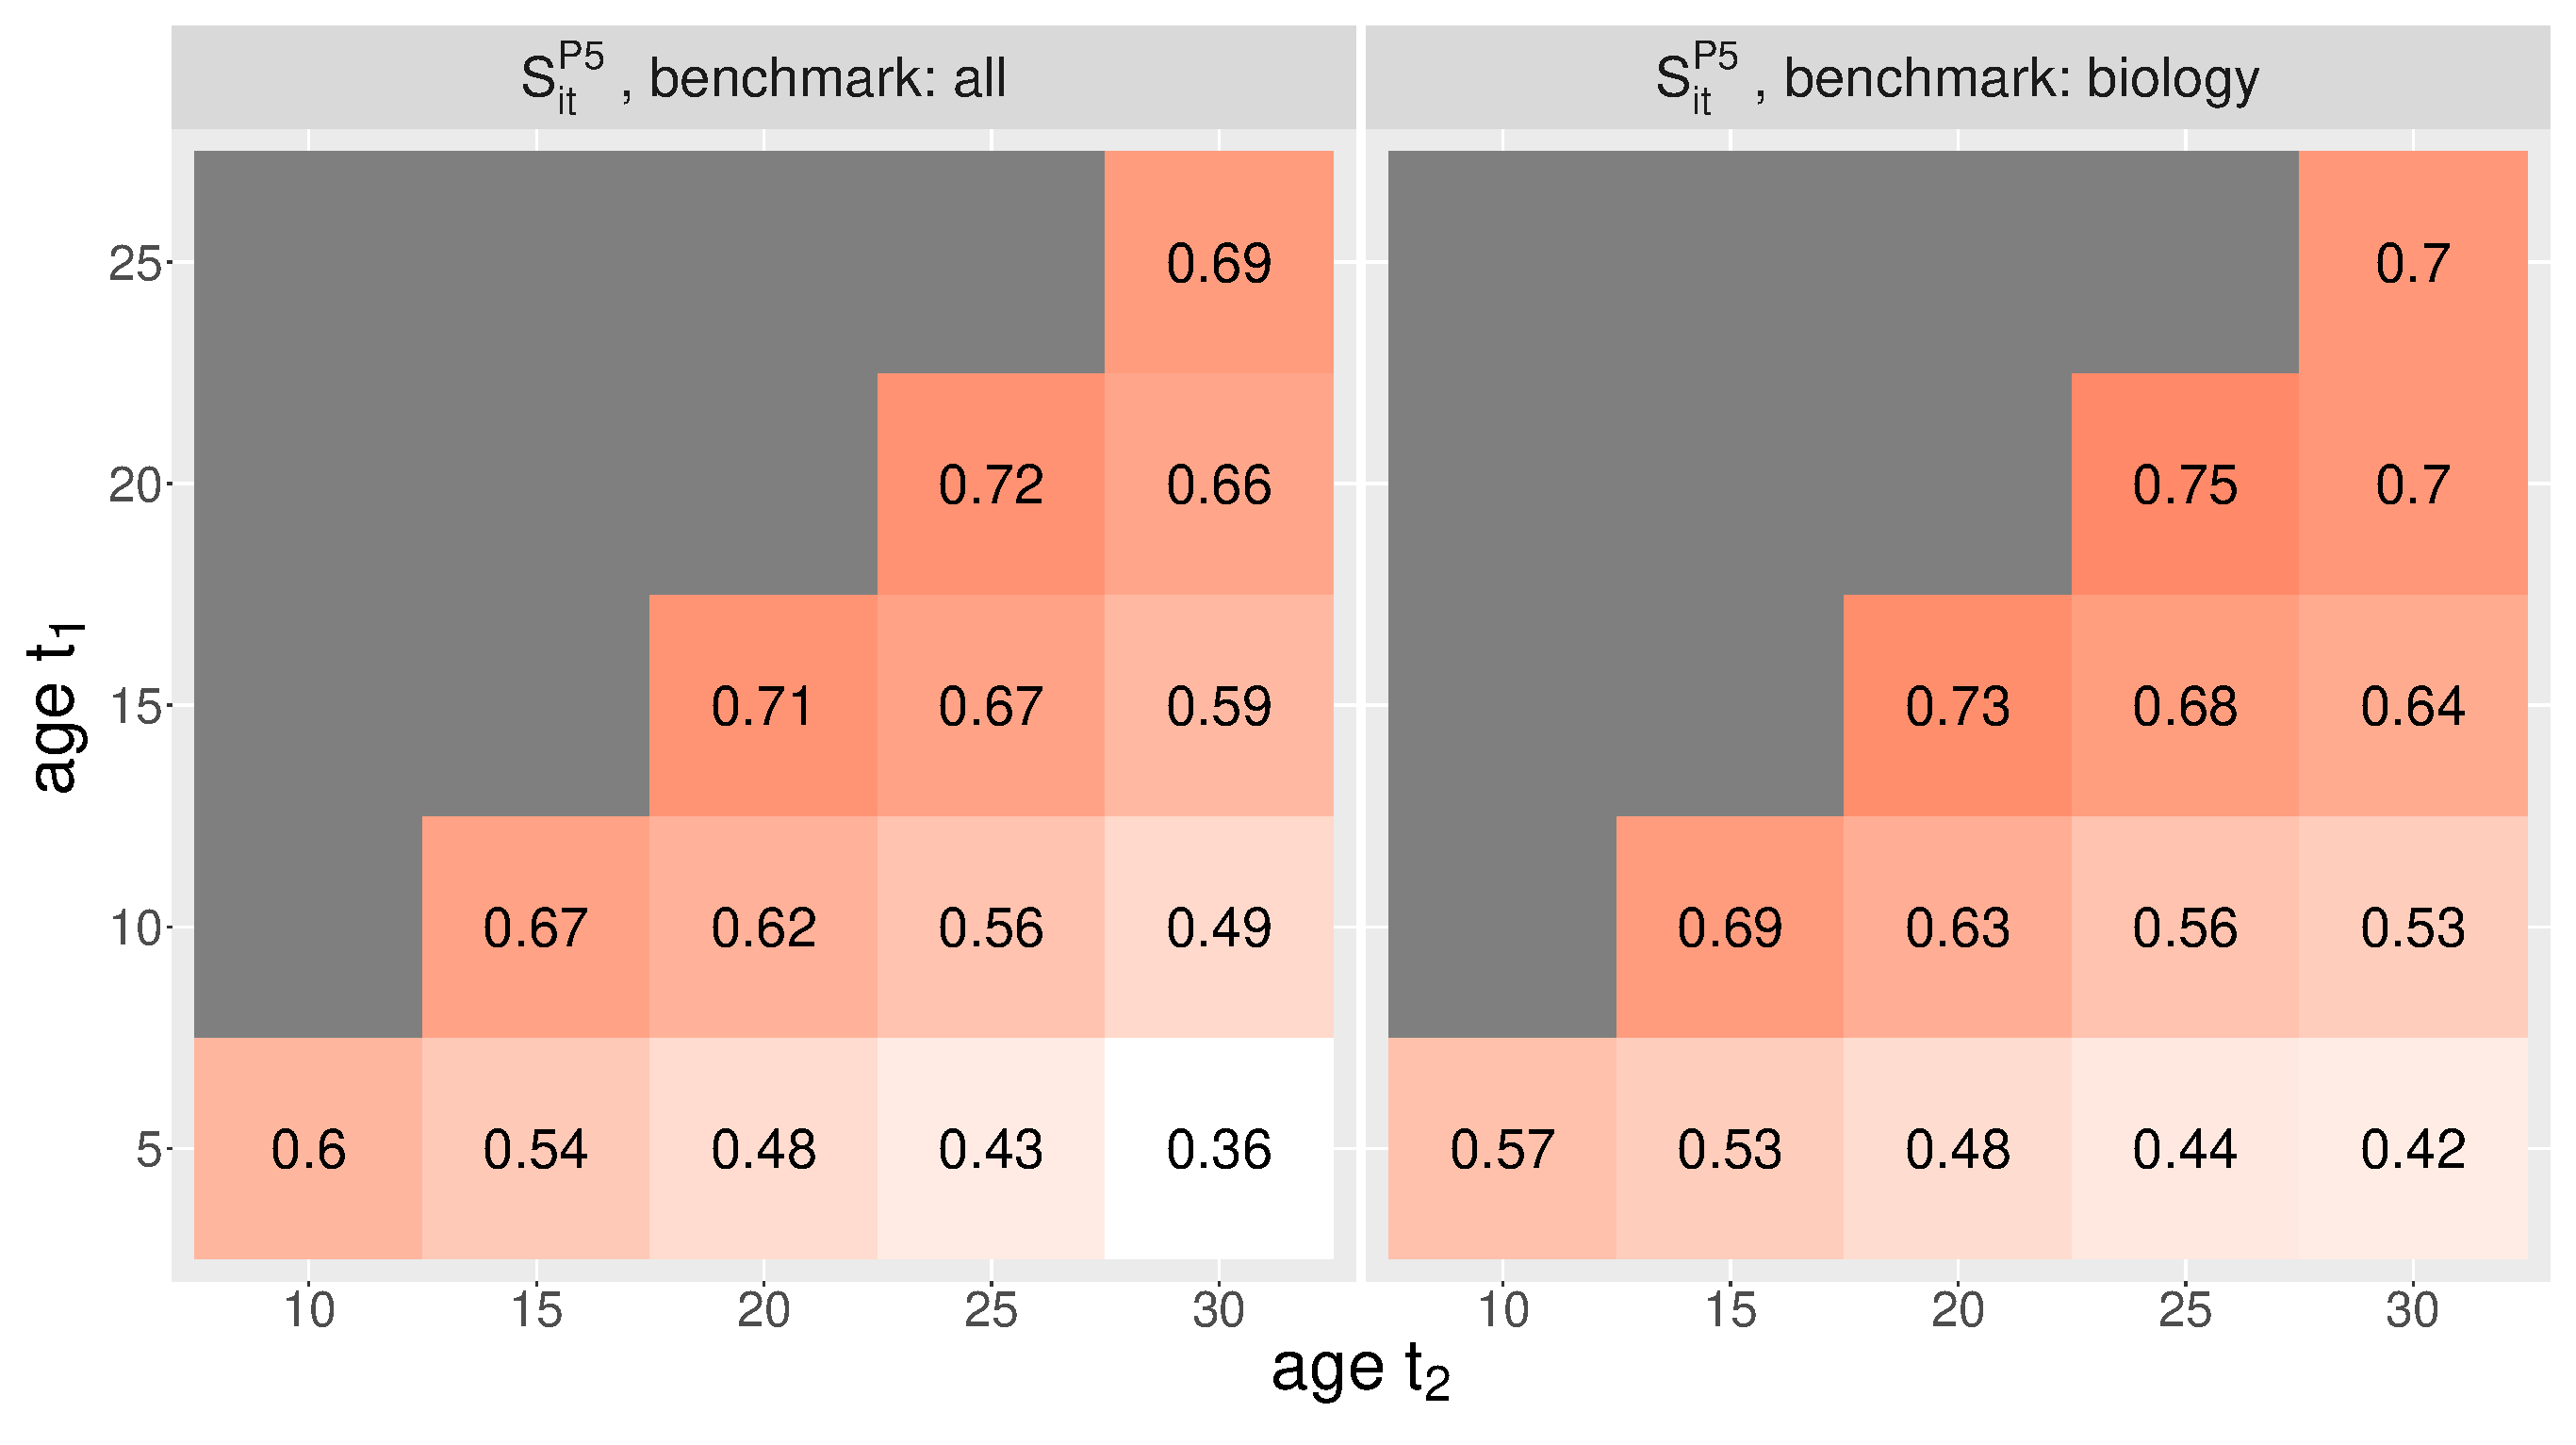
\includegraphics[width=\textwidth]{figures/pred_power/future/heatmap_cor.eps}
         \caption{Predict the future scientific output}
         \label{fig:hm_rp_future}
    \end{subfigure}
    \caption{The Pearson's correlation between RP indicators at two different ages. }
    \label{fig:hm_rp}
\end{figure}
\begin{figure}[ht!]
    \centering
    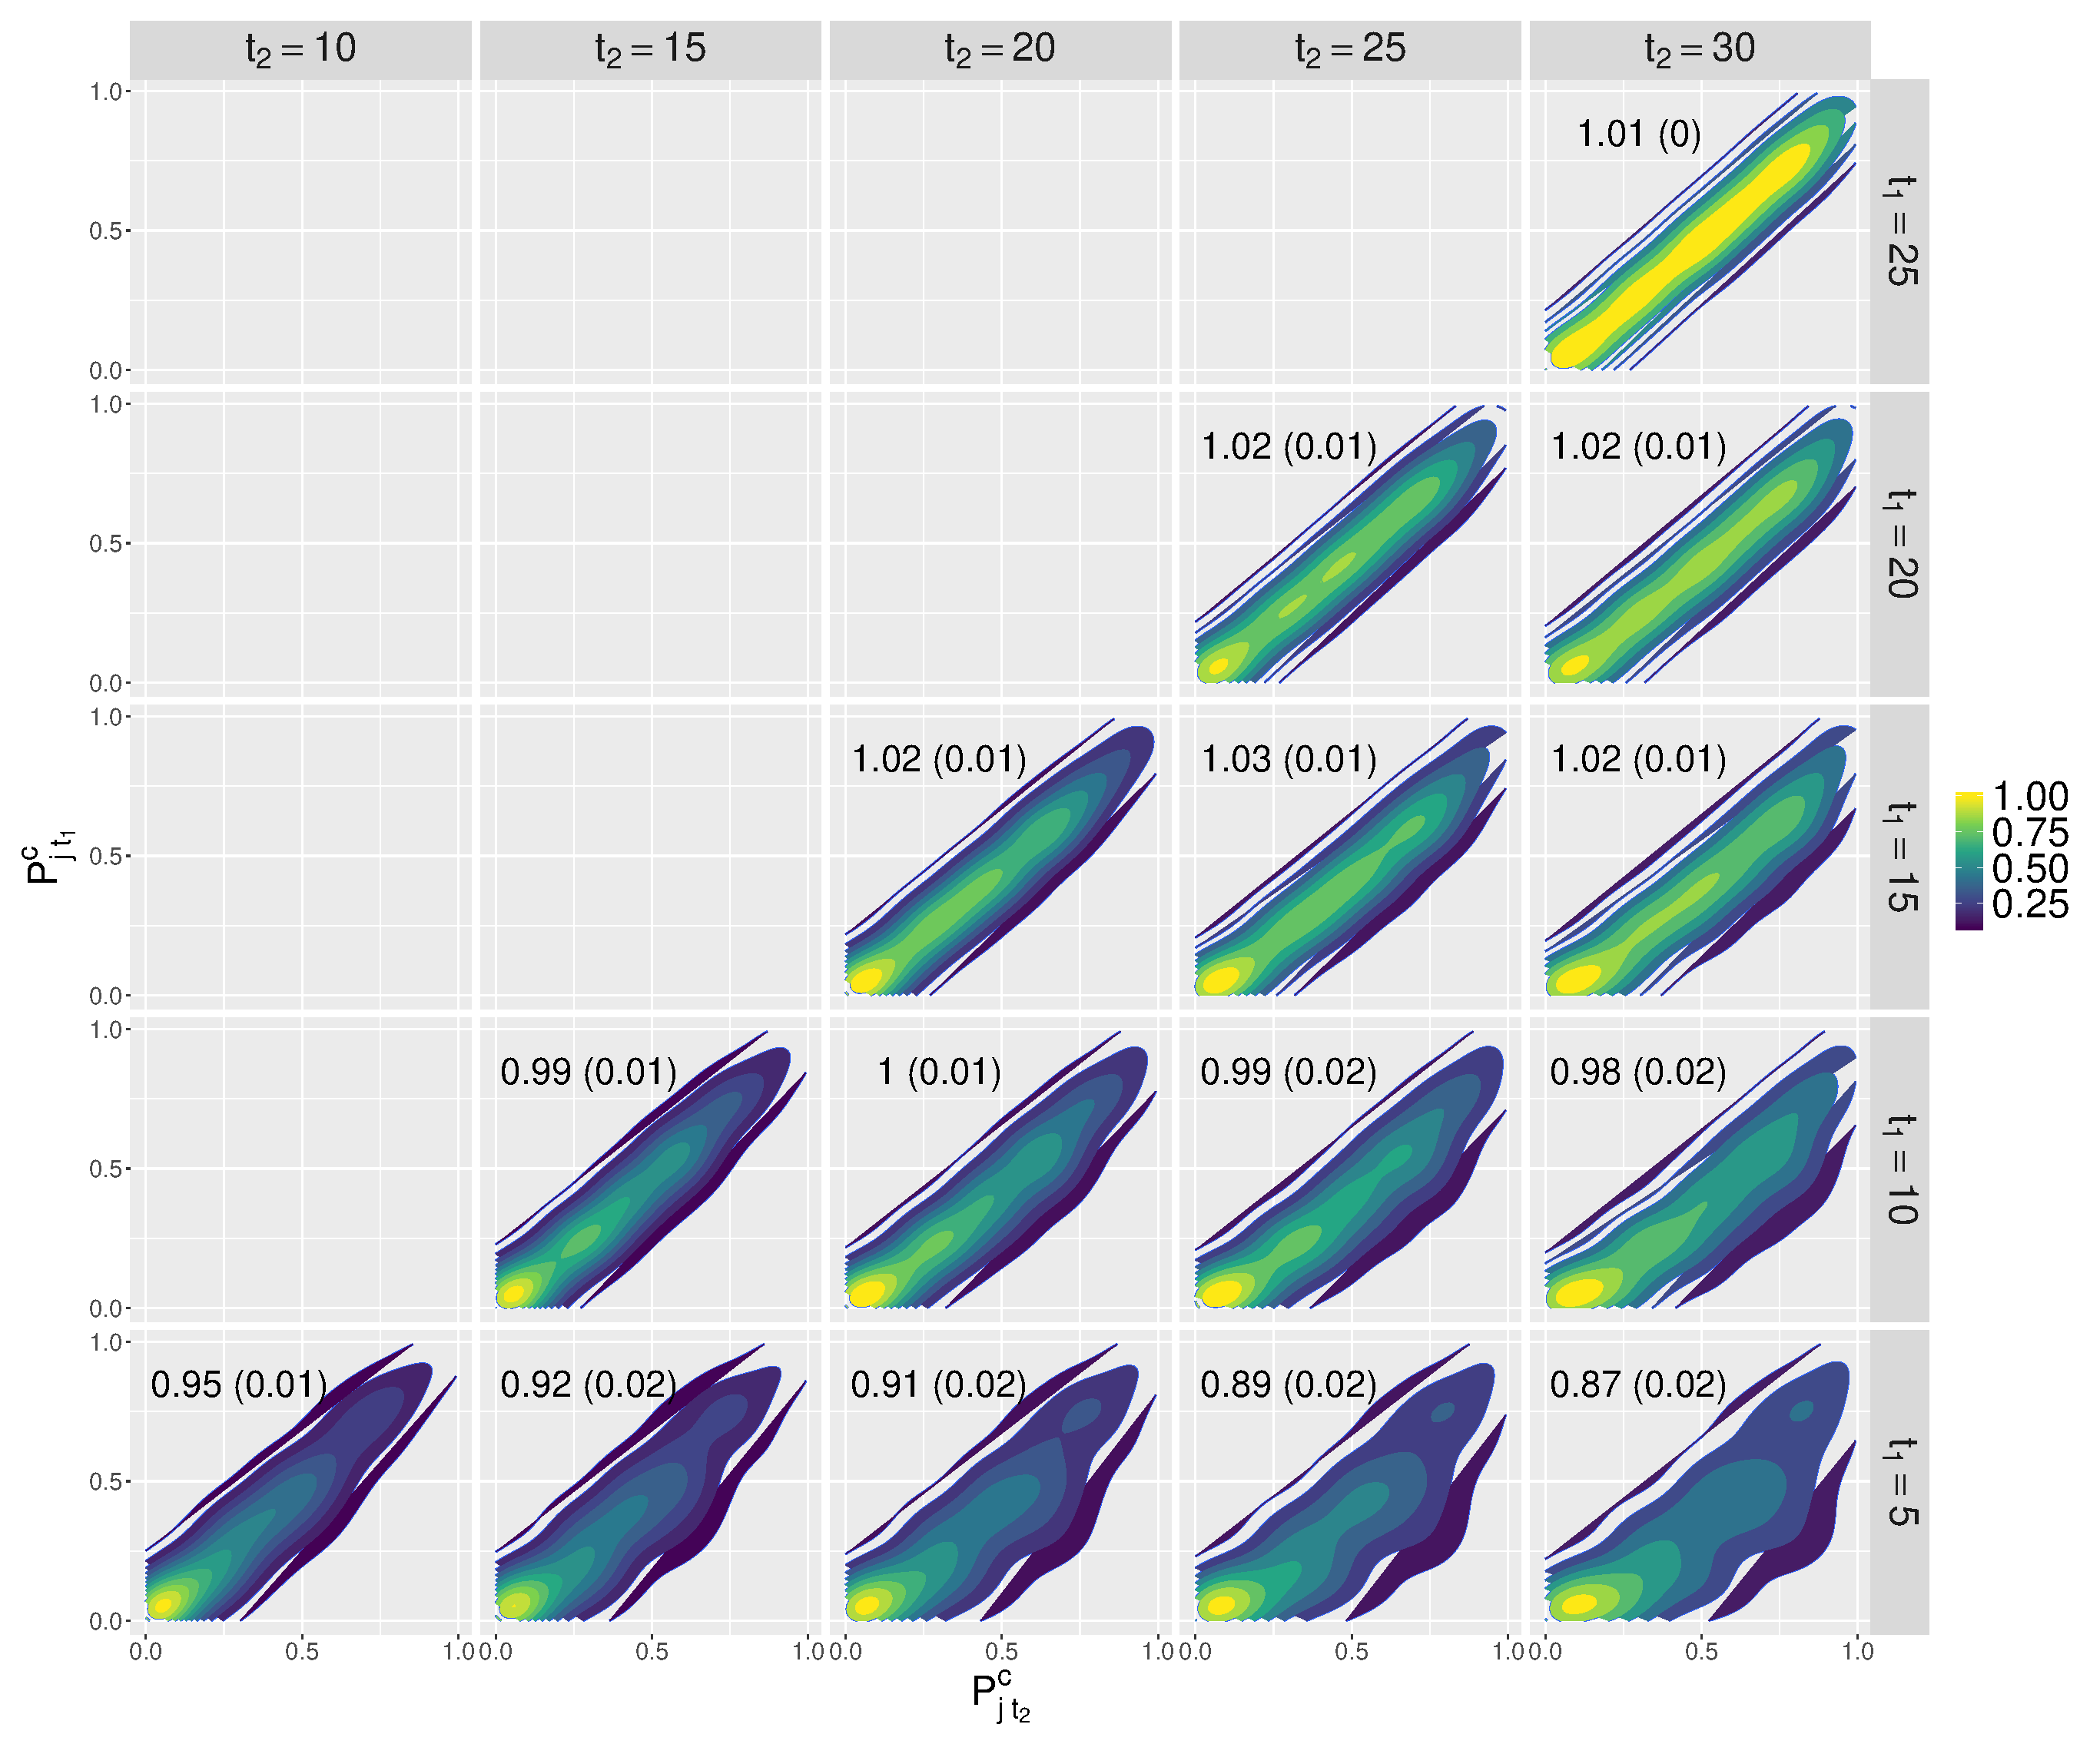
\includegraphics[width=\textwidth]{figures/pred_power/pubrp/scatter_bio1980.eps}
    \caption{Kernel density estimation of the scatters of P$_{j t_1}^c$ and P$_{j t_2}^c$. Meanwhile, we fit a simple linear regression of P$_{j t_2}^c$ upon P$_{j t_1}^c$. The estimated coefficient and the corresponding standard error (in the bracket) are displayed in each facet. The benchmark here includes all publications in biology and written in $1980$.}
    \label{fig:scatter_pubrp_bio1980}
\end{figure}


\begin{figure}[ht!]
    \centering
    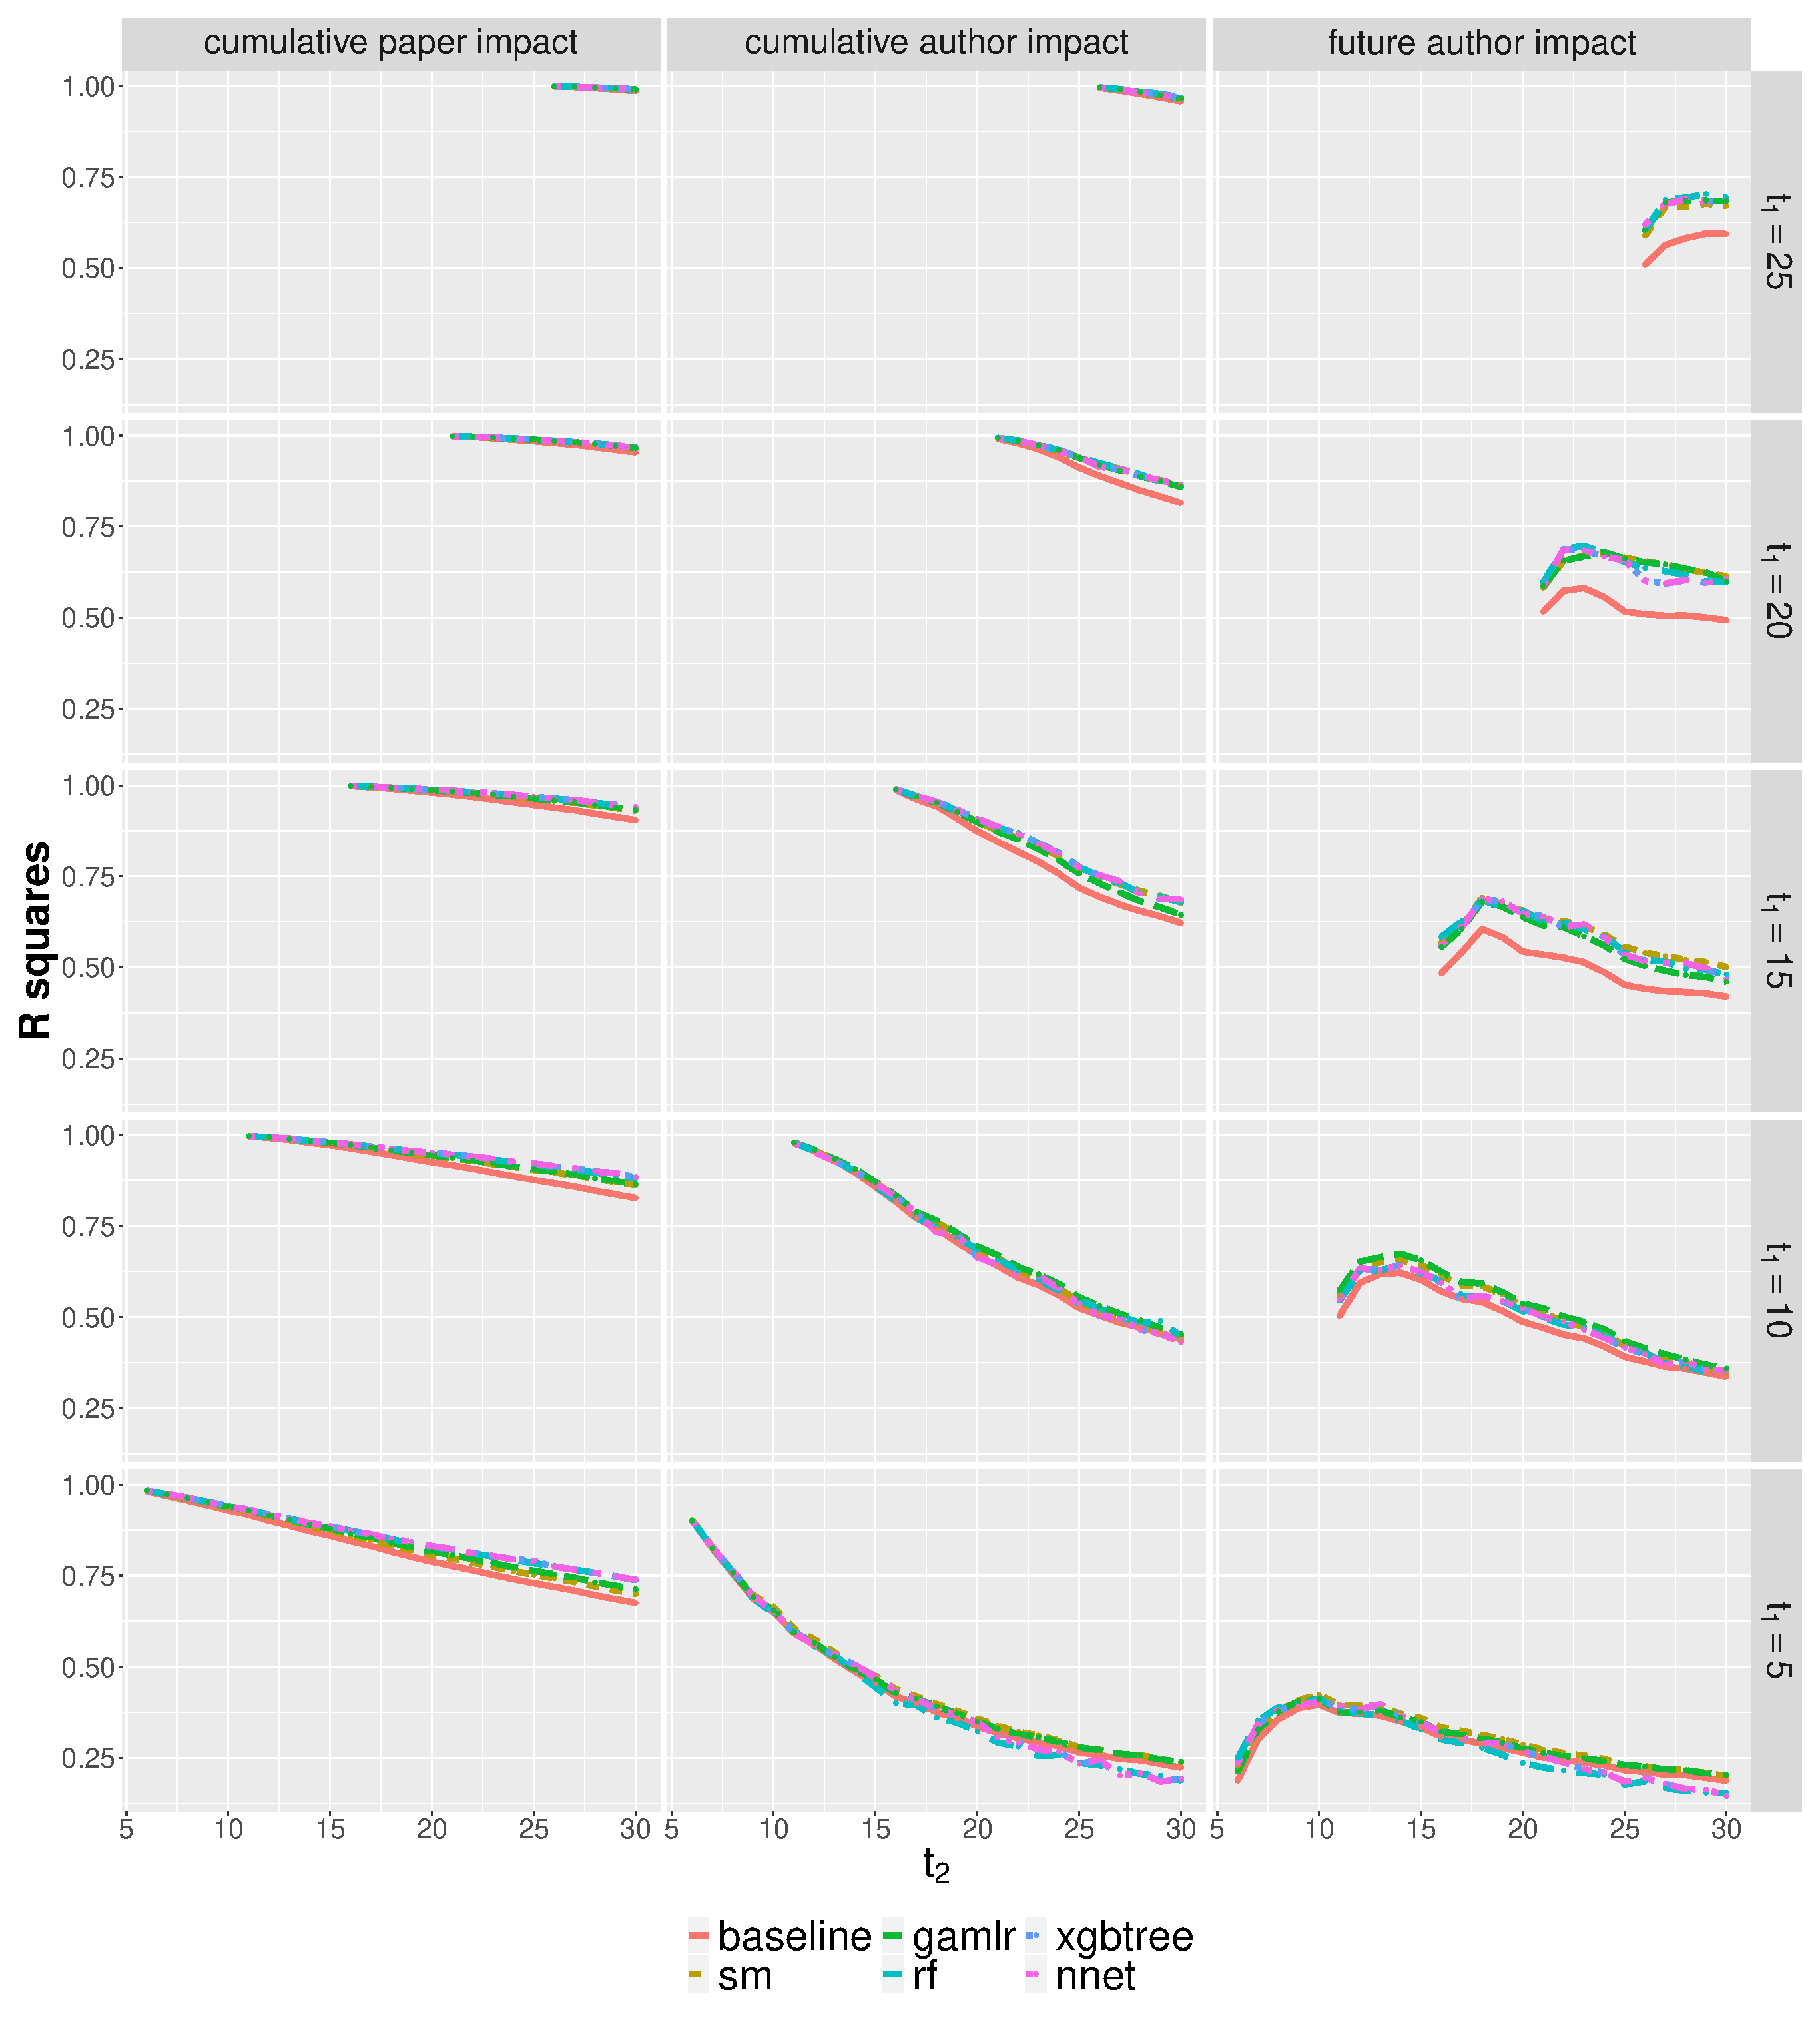
\includegraphics[width=\textwidth]{figures/pred_model/r2_diff.eps}
    \caption{Testing R squares of the predictive models. LASSO, ridge and elastic net are outperformed by Gamma LASSO, and hence are ignored for a better visualization.}
    \label{fig:pred_r2}
\end{figure}


\subsection*{A discussion on various types of rank percentile indicators for scholars}
S$_{it}^{c,b}$, S$_{it}^{h,b}$ and S$_{it}^{P5,b}$ are built upon an aggregation of the performances of the papers that the scholar publish by age $\tau$. S$_{it}^{c,b}$ and S$_{it}^{h,b}$ use the citations $c_{jt}$ to evaluate publication $j$ while S$_{it}^{P5,b}$ uses P$_{j5}^{c,b}$, i.e. the rank percentile of publication $j$ at age $5$. Meanwhile, the aggregation function for S$_{it}^{c,b}$ and S$_{it}^{P5,b}$ is sum, and it's a threshold function for S$_{it}^{h,b}$. 

S$_{it}^{P5,b}$ improves the major drawbacks of the other two indicators. First, it removes the seniority effect of publications, by evaluating the publications by their performances at age $5$. However, both the citations c$_{it}$ and h-index h$_{it}$ are dominated by 'senior' publications and newly published works can hardly contribute. Second, it improves over S$_{it}^{c,b}$ since it hardly rewards authors who publish a large number of low-impact works or only participate in a small number of high-impact projects. Similar to the h-index, the evaluation metric m$_{it}$ of rp.rp5 limits the contribution of a single publication to be at most $1$ due to the definition of rank percentile. However, the absolute number of citations is unlimited and is highly influenced by extreme values. Last, by comparing with rp.h, it penalizes authors who are not truly innovative, but carefully massage their h-indices by publishing a number of papers that are not top-class but attract just enough amount of citations to boost the h-index. As long as a paper is among the top h papers, the actual number of citations is irrelevant for rp.h, but it still affects rp.rp5.

We demonstrate these advantages of rp.rp5 by examining some extreme cases. We create three synthetic academic careers. Author A publishes a substantial number of publications at each age (more than $90\%$ of other authors in the benchmark), while all of the publications have little impacts. Meanwhile, author B and author C only publish $1$ paper at the beginning of their careers, where author B's paper is astonishing while author C's is average. All three authors have h-index as $1$ throughout their careers. Figure \ref{fig:simulated_authors} shows the author rp for these three artificial authors. We see that for author A and B, rp.c is substantially larger than the other two, and it dies down slowly. Even though author B only publishes one ground-breaking paper, the author remains in the top $50\%$ even by age $12$. Both rp.rp5 and rp.h are better characterizing the performances of these authors. Meanwhile, author C has the same rp.h as author B although his/her publication has much less impact. In this case, rp.rp5 and rp.c are better especially at the beginning of the careers. 

Besides these special cases, for the majority of authors in our dataset, we see a large agreement between rp.rp5 and the other two types of rp. Consider the benchmark being biology. In order to study the agreement, for each indicator, we classify the authors into four classes, class $1$: $0\le \text{rp} < 0.25$, class $2$: $0.25\le \text{rp} < 0.5$, class $3$: $0.5 \le \text{rp} < 0.75$ and class $4$: $0.75 \le \text{rp} \le 1$. An agreement in the classification of an author is where two (or three) different rp belong to the same class. The overall agreement for all three rp is $51\%$ at age $5$ and $68\%$ at age $30$, i.e. about half of the authors result in the same classifications of the three rp at age $5$, while that number becomes around two third at age $30$. Figure \ref{fig:aut_rp_class} shows the detailed classifications for every pair of the three rp. As we can see that, the agreement increases with the age. Furthermore, rp.rp5 has large agreements with both rp.c and rp.h, that are $69\%$ and $67\%$ respectively at age $5$, and $71\%$ and $81\%$ respectively at age $30$. 

We've shown the advantage of using rp.rp5 over indicators like rp.c and rp.h. A remaining question is why we use rp.c$_{j5}$ rather than say rp.c$_{j10}$ to represent the quality of the paper. It turns out that rp.c$_{j\tau}$ is highly stable over ages, and rp.c$_{j5}$ is very close to rp.c$_{j10}$ for the majority of papers. This will be discussed in the section below. Therefore, we are using less citation information and get similar accuracies. Other choices involve taking the summary statistic of the entire history of rp.c$_{j\tau}$ ($\tau=1,\cdots,T_j$). For example, we can take the best performance along the history, i.e. $\displaystyle \max_{t=1,\cdots,T_j} \text{rp.c}_{jt}$. We demonstrate that the evaluation metric m$_{i\tau}$ formulated based on these alternatives is highly correlated with m$_{i\tau}$ formulated rp.c$_{j5}$. Furthermore, the rank percentile indicators based on these alternatives are not statistically different from rp.rp5. The details are discussed in the supplemental material section \ref{sec:robustness_rprp}.

\subsection*{Predictive power of rank percentile indicators}
Citations have been shown to lack long-term predictive power\supercite{Wang2013}. Figure \ref{fig:pred_cit_age} shows that publications with the same citations by age $5$, can have noticeably different citation paths and long-term effects. Meanwhile, exceptional and creative ideas can normally take longer to be appreciated by the community. As shown in figure \ref{fig:pred_cit_cit}, the correlation between short-term citations and long-term citations breaks down for most highly-cited papers (the shaded area). Such problems affect less for rank percentiles, as evidenced by figure \ref{fig:pred_rp_age} and \ref{fig:pred_rp_rp}. For the papers having rp.c$_{j 5} \approx 0.75$, their rp.c$_{j 30}$ are all above $0.5$. Meanwhile, the correlation between short-term and long-term rp is still very strong for the most highly-cited papers. 

Publication rp.c$_{j\tau}$ and scholar rp.rp5$_{i\tau}$ are highly predictive and stable over age. Figure \ref{fig:hm_rp_current} shows the ability of the indicators to predict their own values. We see an extremely high predictive power for rp.c, which indicates that a publication with high rp.c after $\tau_1$ ages is very likely to have high rp.c after $\tau_2$ ages where $\tau_2 > \tau_1$. Meanwhile, the predictive power dies down as the forecast horizon gets larger, which simply reflects the difficulty of long-term forecast. Also, the correlation becomes higher when we have a longer history of the publication, e.g. it increases from $0.79$ to $0.86$ as $\tau_1$ changes from $5$ to $10$ while keeping the forecasting horizon fixed at $\tau_2-\tau_1=5$. Finally, we see a slightly higher predictive power when we restrict the benchmark to only include publications in biology.

Similar patterns can be observed for rp.rp5 according to figure \ref{fig:hm_rp_current}, although it has lower predictive power than rp.c. To be more specific, it starts with a high predictive power but dies down fast as the forecast horizon becomes larger. For instance, the correlation drops from $0.99$ to $0.94$ for rp.c while it decreases from $0.94$ to $0.77$ for rp.rp5, by fixing $\tau_1=15$. This is result from the fact that forecasting future impact of future works is considerably harder than forecasting the future impact of existing works. Predicting rp.c$_{j\tau_2}$ belongs to the latter. On the other hand, rp.rp5$_{i\tau_2}$ is based on the set of papers that scholar $i$ publishes by age $\tau_2$, which contains papers published by $\tau_1$ and papers published in the period of $(\tau_1,\tau_2]$. Hence, predicting rp.rp5$_{i\tau_2}$ involves predicting the future impact of existing works as well as the future impact of future works. As the forecast horizon $\tau_2-\tau_1$ becomes larger, we potentially have more `predicting the future of future' to deal with that makes the task tougher. Meanwhile, other types of scholar rank percentile indicators, rp.c and rp.h, have very similar predictive powers with rp.rp5, which is illustrated in figure \ref{fig:hm_autrp_current}.

It turns out that not only do publication rp.c has high predictive power, it's stable over age, i.e. rp.c$_{j\tau_1}\approx$rp.c$_{j\tau_2}$. Figure \ref{fig:scatter_pubrp_bio1980} shows the kernel densities of the scatters of rp.c$_{j\tau_1}$ vs rp.c$_{j\tau_2}$. We see that the scatters are mostly along the $45$ degree line. Meanwhile, we perform a simple linear regression by regressing rp.c$_{j\tau_2}$ upon rp.c$_{j\tau_1}$. The regression coefficient of variable rp.c$_{j\tau_1}$ together with the standard error is displayed besides each of the scatters in the figure. We see that the coefficients are very close to $1$ with very small standard errors, which gives further evidence that rp.c is stable over age. Meanwhile, figure \ref{fig:scatter_autrp_all} shows a similar study for the stableness of rp.rp5. We do not see strong evidence of rp.rp5 being stable over age.

We know that predicting rp.rp5 involves forecasting the future impact of both existing and future works. Such question can assist making decisions for a faculty position or tenureship, since the committee would like to examine the cumulative scientific impact of the scholar. A more difficult question is to predict the future impact of the future works. Such question is of interest, for example, in assigning research fundings or allocating research resources, where the future impact of existing works shall be irrelevant. Figure \ref{fig:hm_rp_future} shows the ability of using rp.rp5$_{i\tau_1}$ to predict rp.rp5$_{i\tau_2 \setminus \tau_1}$, where the latter is based on only the future papers, i.e. those written in the $(\tau_1,\tau_2]$ time interval. As expected, we see lower a predictive power than predicting rp.rp5$_{i\tau_2}$, but rp.rp5$_{i\tau_1}$ can still explain most of the variations in rp.rp5$_{i\tau_2 \setminus \tau_1}$ in relatively short horizons. 

\subsection*{Predictive models}
For both the publication and scholar impact, we've studied how well the performance by age $\tau_1$ predicts the cumulative achievement by age $\tau_2$. We demonstrate that rank percentile indicators (rp.c$_{j\tau}$ and rp.rp5$_{i\tau}$) have high predictive powers. Meanwhile for the scholar impact, we further investigate the prediction of performance in the subsequent $\tau_2-\tau_1$ ages, i.e. using rp.rp5$_{i\tau_1}$ to predict rp.rp5$_{i\tau_2 \setminus \tau_1}$. 

We now formulate these prediction tasks as supervised learning problems, and examine how much improvement we can get by having an extensive list of features and complex fitting algorithms. We consider the following fitting procedures; these models are ordered by increasing complexity, starting from simple baselines and ending with complex machine learning models:
\begin{itemize}
    \item Baseline: a simple linear regression of rp$_{\star \tau_2}$ upon rp$_{\star \tau_1}$.
    \item Simple Markov model (sm): a linear regression model of rp$_{\star \tau_2}$ upon features only including rp$_{\star \tau_1}$ and the change of rp over the last $2$ ages.
    \item Penalized linear regression models, including ridge\supercite{hoerl1970ridge}, LASSO\supercite{tibshirani1996regression}, elastic net (enet)\supercite{zou2005regularization} and the Gamma LASSO (gamlr)\supercite{taddy2017one}: linear models with different penalties on the regression coefficients. All of these methods shrink the coefficients towards zero, and the later three methods can provide sparse solutions (shrink the coefficients to exactly zeros). 
    \item Ensemble methods of regression trees, including random forest (rf)\supercite{liaw2002classification} and extreme gradient boosting trees (xgbtree)\supercite{chen2016xgboost}: rf is a bagging of regression trees with a subset of randomly selected features chosen at each split to avoid overfitting. xgbtree is a fast implementation of gradient boosting on regression trees with a model formation that emphasizes the role of regularizations to avoid overfitting.
    %\item Support vector regression (svr)\supercite{drucker1997support}: 
    \item Deep neural networks (dnn): feedforward networks with multiple hidden layers and using dropout and $l_2$ regularization to avoid overfitting.
\end{itemize}

\subsubsection*{Features and model fitting}
A crucial step for supervised machine learning models is feature engineering. The features that we create are based on the citation histories and are characterized into either author related or paper related features. For example, to predict the author impact rprp5$_{i\tau_2}$, an author related feature can be the number of papers that the author publish by age $\tau_1$, and a paper related feature can be the average citations of these papers. The $30$ features for predicting the publication impact and the $42$ features for predicting the author impact, are listed in tables \ref{tab:features_pubrp} and \ref{tab:features_autrp} respectively. 

The features are created only using the citation information available by $\tau_1$ and the response is specified at $\tau_2$. With a pair of features and response, all the models are trained and evaluated on the testing set, where the training and testing are randomly split in a 9-1 ratio. We consider $5$ different values of $\tau_1$ representing different stages of a publication or a scholar, that are $\tau_1\in\{5,10,15,20,25\}$, and for each $\tau_1$ we have $\tau_2=\tau_1+1,\cdots,30$, which results in $75$ pairs of $(\tau_1,\tau_2)$ in total. Hence all the models are trained $75$ times independently. Meanwhile, the machine learning models all rely on some hyper-parameters that require careful tuning. We use randomized searching with multiple iterations over a pre-specified parameter space, and the optimal set of hyper-parameters is chosen to minimum the 10-fold cross-validation error.

If we ignore the fact that we are modeling rp.c$_{j\tau}$ and rp.rp5$_{i\tau}$ at fixed time points, and view them as time series. Both series turn out to be non-stationary, based on statistical tests such as the Dicky-Fuller test\supercite{dickey1979distribution} and the KPSS test\supercite{kwiatkowski1992testing}, where the details are discussed in the supplemental material section \ref{sec:stationarity_test}. It's often encouraged to work on stationary series, for example in the autoregressive and moving average models, and a typical practice is to model differenced series. We follow the same logic here, and use the differenced series as the responses, e.g. $\Delta \text{rp.c}_{j\tau_2} = \text{rp.c}_{j\tau_2} - \text{rp.c}_{j\tau_1}$. 

\subsubsection*{Results}
We consider four evaluation metrics for the predictive models, that are the R squares ($R^2$), root mean squared error (RMSE), root median squared error (RMEDSE) and mean absolute error (MAE). The $R^2$ for all the models are shown in figure \ref{fig:pred_r2}, while the rest of the metrics are displayed in figure \ref{fig:pred_rmse}, \ref{fig:pred_medse} and \ref{fig:pred_mae}. We see that the baseline model predicts the cumulative impacts well, and the improvement of using more features and machine learning models have little benefit. Meanwhile, the baseline model can still provide reasonable predictions for the future scholar impact, although the machine learning models can provide better results when $\tau_1$ is relatively large. However, in such scenarios, the simple Markov model performs closely to the machine learning models, and hence the extensive list of features and complex non-linearity have little impact.





